\chapter{Simultaneous Multiple Surface (SMS) 2D Designs as Starting Points for Lens Optimization} %% change
\label{chapter_5_SMS} %% change
\graphicspath{ {./chapter-5/figures/} }  %% change
\captionsetup[figure]{labelfont=bf}
\captionsetup{margin=1.5em}
\captionsetup[table]{labelfont=bf}
%% The following annotation is customary for chapter which have already been
%% published as a paper.
\blfootnote{Parts of this chapter have been published in Optics Express \textbf{25}, 32474 (2018) \cite{HouSMS2018}.}

%% It is only necessary to list the authors if multiple people contributed
%% significantly to the chapter.
%\authors{Albert {\titleshape Einstein}}

%% The '0pt' option ensures that no extra vertical space follows this epigraph,
%% since there is another epigraph after it.
% \epigraph[0pt]{
%   A journey of a thousand miles begins with a single step
% }{Laozi}

% \epigraph{
%     Sample quotes
% }{author}

% \begin{abstract}
% Previous researches have shown that different solutions of the optical system can be found using saddle point based method for some simplified cases\cite{PascalTriplet2009}. It is important, however, to study whether the saddle point based method still perform well in practical lens design problems. To study this, we chose to start with a relative simple example.
% \end{abstract}

% %% Start the actual chapter on a new page.
% \newpage

\noindent 


%%%%%%%%%%%%%%%%%%%%%%%%%%%%%%%%%%%%%%%%%%% Section 1 %%%%%%%%%%%%%%%%%%%%%%%%%%%%%%%%%%%%%%%
\section{Introduction}
% repeat how the optical is done conventionally. Simple systems are determined by forward model analysis. The result from the simple model is then used as starting point for designing systems with more complexity.  
Choosing a sufficient good staring configuration is crucial to every kind of optical design. For a simple systems requiring a limited amount of optical elements, analytical method such as paraxial calculation or aberration analysis can be used to determine a starting point. For systems with demanding requirements (e.g. larger FOV, high image quality) it is usually more convenient to select a starting configuration based on existing designs documented either in lens design books \cite{book:Kingslake}\cite{book:SmithModernOpticalEngineering}\cite{book:FisherOpticalSysDesign} or in various patents. Once the starting point is determined, the system is parameterized in a design software and further improved in order to fulfill various constraints and performance requirements. In most cases, additional degrees of freedom are needed to enhance the system performance. 

The most typical approach in conventional lens design to add degree of freedoms is to introduce new lens elements. We have shown in the previous chapters that one aspect of the Saddle Point Construction (SPC) provides a systematic and rapid approach to improve system performance by adding new lens element. However, adding new elements in the system usually means bigger volume and higher cost, which are disadvantages for practical applications. 
%https://www.osapublishing.org/optica/fulltext.cfm?uri=optica-8-2-161&id=447006 freeform review
% Talking about the other aspect of the work 
Besides using additional lens elements, another way is to introduce new degrees of freedom on existing lens surfaces. For rotational symmetric systems, aspheric surfaces can be used instead of spherical surfaces. For non-rotational symmetric systems, freeform surfaces (surfaces with arbitrary shape) can be used. They permit new dimensions in optical performance by eliminating aberrations without added weight and size, thus fulfilling the need for an ever-increasing performance balanced with an equal desirable goal of ever smaller and lighter optics. Experience shows that aspheric and freeform surface are often more challenging to manufacture and incorporate into design than the conventional spherical surfaces because of their complex geometric shape. Nonetheless, provided the added benefit, the development of precise manufacturing techniques makes aspheric and freeform surfaces no longer a luxury and therefore can be encountered quite often in modern designs. In this chapter, we would like to focus on the aspheric surface since it shares more similarity with spherical surfaces. Freeform will not be discussed. 

% continue to discuss the design with aspheric surfaces
% traditional technique, requirement
%% chain of reasoning!!! 
% mild asphere -> many aspheric parameter -> may trap in LM
% mild asphere -> does not modify the system much -> may trap in the LM already defined by the spherical system -> mild asphere only solves a local issue, it does not fully make the system out of the LM
%%In this approach, the aspheric surfaces may improves the system performance by bring down the merit function. However, if the original spherical design is already in a sub-optimal local minimum, adding aspheric surface is not likely to drastically improve the system performance. 

In common practices, the aspheric surfaces are created by unitizing the existing surfaces of an already designed spherical systems. The designer chooses which surface to be aspherized based on his/her observation. The introduced aspheric surface is then often a "mild" surface, which is described by a small polynomial order. However, if the performance improvement of system is not as expected, the designer may consider using more polynomial terms or choose more surfaces to be aspherized. The increasing choices of the degrees of freedom often trap the system in a poor local minimum (Figure \ref{fig: fig1_landscape}(a))). In such cases, the designer´s experience is often a crucial factor when trying to get out of a poor minimum in search for a good solution. In the case of utilizing aspheric surfaces, the aim is to add the correct design freedoms such that the new starting point with more degrees of freedom can lead to better system performance (Figure \ref{fig: fig1_landscape}(b)). %create starting points in higher dimensions 
%% describing the sequence of using variables affects the results since there is no control on the basin of attraction it stays. 

%% 05-19 regarding the optimization algorihm mentioned that it is an optimization approach (inverse problem) . 1) for aspheric case, it is also possible to use all the generic global optimizer -> brute force method by freeing a lot of freedom and then optimize 2) alternatively, using a physical insight to construct the aspheric surfaces, and trust it to be in a good basin and do local optimization.
%在动态的system design变化中,因为有多design 步骤,landscape会变化很多,所以large chance不在一个好的basin里。 设计思路:减少design steps, 减少那些会很大程度上改变design landscape的步骤,或者每次有大的改变,要重新anchor back to a good basin。
% 有些解是在加了complexity之后才出现的(freedom, constraint),这些indicate 我的本来的问题(merit function)已经可能发生了变化 -> 问题的性质发生了变化

Several global optimization methods such as genetic algorithms \cite{Moore1999}, evolution strategies \cite{Nagar:18}, particle swarm \cite{MenkeParticleSwarm} and simulated annealing \cite{Forbes1991} have been adapted to different optical design problems to avoid getting trapped in a local minimum. One can add the aspheric variables to the existing ones and run a global optimization to find out what the could be the best performance. However, these methods are based on generally applicable mathematical models, and designers understand little about the optical systems behind them. 
%Another method known as saddle point construction (SPC) method uses a systematical approach to find solutions in the design landscape and helps to get out of bad local minima \cite{BociortSPCSexplained}\cite{HouSimple16}.
%% back in discussing these optimization method again
 
\begin{figure}[h!]
    \centering
    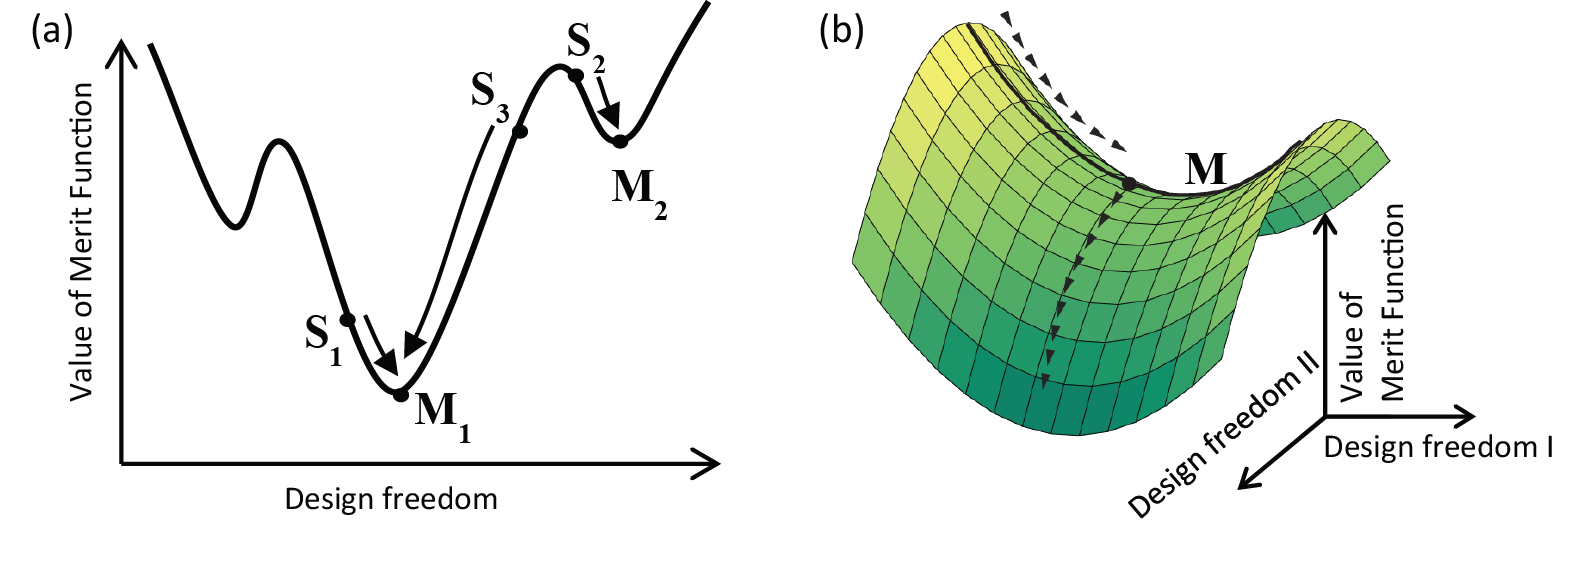
\includegraphics[width=0.8\textwidth]{chapter-5/figures/Figure1_landscape.png}
    \caption{An illustration of an design landscape in 2D (a) and 3D (b). The plot (a) on the left shows that the obtained local minimum is sensitive to the starting point: Choosing $S_2$ as the starting point leads to a sub-optimal local minimum $M_2$, while choosing $S_1$ and $S_3$ leads to a better local minimum. The plot (b) on the right shows that by adding the right design freedom, a local minimum $M$ in lower dimension can progress further to improve system performance.}
    
    \label{fig: fig1_landscape}
\end{figure}
%% different than optimization method, SMS is a way to determine a starting point directly  with aspheric surfaces. 
Alternatively, for non-spherical systems, direct design methods such as the Simultaneous Multiple Surfaces (SMS) method allow to find a better starting point (like S1 in Figure \ref{fig: fig1_landscape}(a)) \cite{WangThesis}\cite{LinWang12OE} and subsequently progress with it with a single step optimization (varying all parameters). Even though SMS is capable of designing good aspheric imaging systems, there is no study comparing it directly with other design strategies and describing the characteristics of different methods.

%Consider the context in this chapter. 
In this chapter, we consider rotationally symmetric designs, for which SMS 2D is used \cite{book:ChavesNonimagingOptics}. SMS 2D may utilize rays in the meridian plane or skew rays \cite{LinWang2011}, but, in any case, obtaining a 2D profile of the surfaces. The method involves simultaneous calculation of N optical surfaces using N one-parameter bundles of rays for which specific conditions are imposed. The number of ray bundles can be greater than the number of surfaces to design when the footprints of the design bundles do not occupy the full SMS surfaces. This can be controlled by the size of the aperture stop or the relative distance between the aperture stop and the optical surfaces as demonstrated in \cite{BenitezSPIE2014}\cite{FDuerrOE2013}\cite{FDuerrOE12}. SMS also has a freeform version called SMS 3D. However, these cases are not discussed in this paper. 
We start by briefly describing the SMS method applied in this paper. Then the design obtained with SMS is used as a starting point, followed by a single-step optimization of all parameters. The final design is compared with other designs obtained using spherical starting point and single-step, two-step, stepwise and global optimizations. Two designs are considered, a simple one and a slightly more difficult one, with a larger aperture and wider field.
%%%% come back to check later 2021/03/02%%%%%%%%
\section{Starting Point with the SMS Method}
The standard SMS procedure for designing aspheric surfaces involves only meridian rays. It consists of two steps: selection of central segments of the surfaces and recursive generalized Cartesian oval calculation \cite{LinWang2011}\cite{MinanoOE09}. We will focus on SMS designs using only meridian rays. Skew rays are then controlled in a subsequent optimization. 

The illustration in Figure \ref{fig: sms_2d_explain} gives an example of how SMS works. The figure shows one of the approaches on how to design a two-surface aspheric imaging system. The following aspects need to be defined as the starting conditions: 1) Coordinates of the object points (\textbf{O1} and \textbf{O2}) and image points (\textbf{I2} and \textbf{I1}). The points in each pair are symmetric to each other with respect to the optical axis. 2) Vertex position (\textbf{P0}) of one of the surfaces and its normal (along the optical axis); thickness of the lens (it is approximated by the projection of \textbf{P0-P1} on the optical axis in Figure \ref{fig: sms_2d_explain}). 3) The refractive indices of the lens (\textit{n'} and the medium outside the lens \textit{n0}). 

With all the above parameters defined, the SMS starts with tracing the ray from \textbf{O1} to \textbf{P0}. Then the ray is refracted to \textbf{P1}, then to \textbf{I1}(the normal at \textbf{P1} can now be calculated). Once the first complete ray is traced from \textbf{O1} to \textbf{I1}, the optical path distance (OPD) from \textbf{O1} to \textbf{I1} is determined. Because of the symmetry, a perfect imaging system will produce the OPD from \textbf{O2} to \textbf{I2} identical to that from \textbf{O1} to \textbf{I1}. When tracing the ray from \textbf{I2} to \textbf{P1}, the refracted angle of the ray is known. Given the OPD and the end point as \textbf{O2}, the position of \textbf{P2} and the local normal can be calculated. 

Now, it is clear that the next step would be tracing the ray from \textbf{O1} to \textbf{P2}. The aforementioned steps can be iterated such that a chain of points is constructed. These points are positioned sparsely on the chain. To get dense sampled points, a curve can be interpolated with two neighboring points (e.g.  \textbf{P0} and \textbf{P2}) and their normals. A new point can be selected on this curve with its normal. Starting with the new point, we can perform the ray-tracing step again to create denser sampled points filling the gap between the original two points. The same procedure can be repeated with all the sparse points firstly created. After the dense sample points are available on both sides, surfaces can be created by fitting these points. 

This is only a brief explanation to show the concept of SMS. More details on different techniques for starting conditions, surface fitting and constructions are well explained in \cite{book:ChavesNonimagingOptics}.

\begin{figure}[h!]
    \centering
    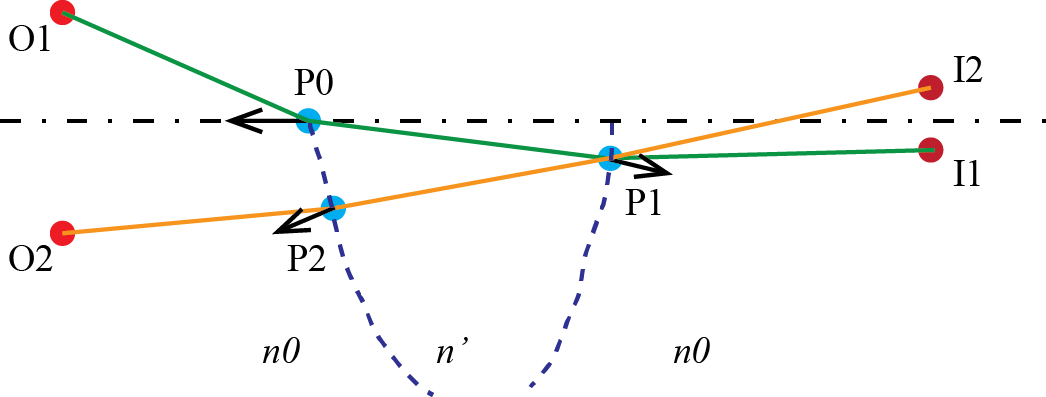
\includegraphics[width=0.85\textwidth]{chapter-5/figures/Figure_sms_explain_2D.png}
    \caption{Illustration of an SMS process to simultaneously construct two surfaces. \textbf{O1} and \textbf{O2} are pre-selected points on the object side. \textbf{I1} and \textbf{I2} are the ones on the image side. \textbf{P0} - \textbf{P4} are the examples of the constructed points which are used to build the optical surfaces. Arrows indicate the direction of the surface normal at each point. }
    \label{fig: sms_2d_explain}
\end{figure}

In this chapter, two designs are studied. Both designs consist of four aspheric surfaces. The two designs are distinguished by the F/Number (aperture size) and the FOV where a smaller F/Number and larger FOV is considered as a more demanding design. With the SMS 2D approach, four meridian bundles were used. It is different from the two surfaces case in the way that the starting conditions include the parts of the surfaces near the axis, which are calculated with paraxial optics \cite{MinanoOE09}. In the case at hand, the four meridian ray bundles selected for the SMS design correspond to the rays emitted from four object points placed symmetrically with respect to the optical axis at infinity. The image points are located in the same way at a finite distance to match the specified focal length. The field angles associated with the object points are selected so that their root mean square 2D (RMS2D) distribution curves (defined as the RMS spot diameter calculated using only meridian rays in the field) present a ripple shape over the field of view as shown in the right-hand plot in Figure \ref{fig: fig2_SMSdesignedSys} and explained in detail in \cite{LinWang12OE}. 

Applying a standard SMS 2D procedure, for the design directions we simultaneously calculate the set of points and normals. SMS profiles are then fitted into a Forbes Qcon polynomial \cite{ForbesOE07}, and parameterized in the CODE V software. This system is now ready to be optimized for the whole field of view, as in the example shown in Figure \ref{fig: fig2_SMSdesignedSys}. 

\begin{figure}[h!]
    \centering
    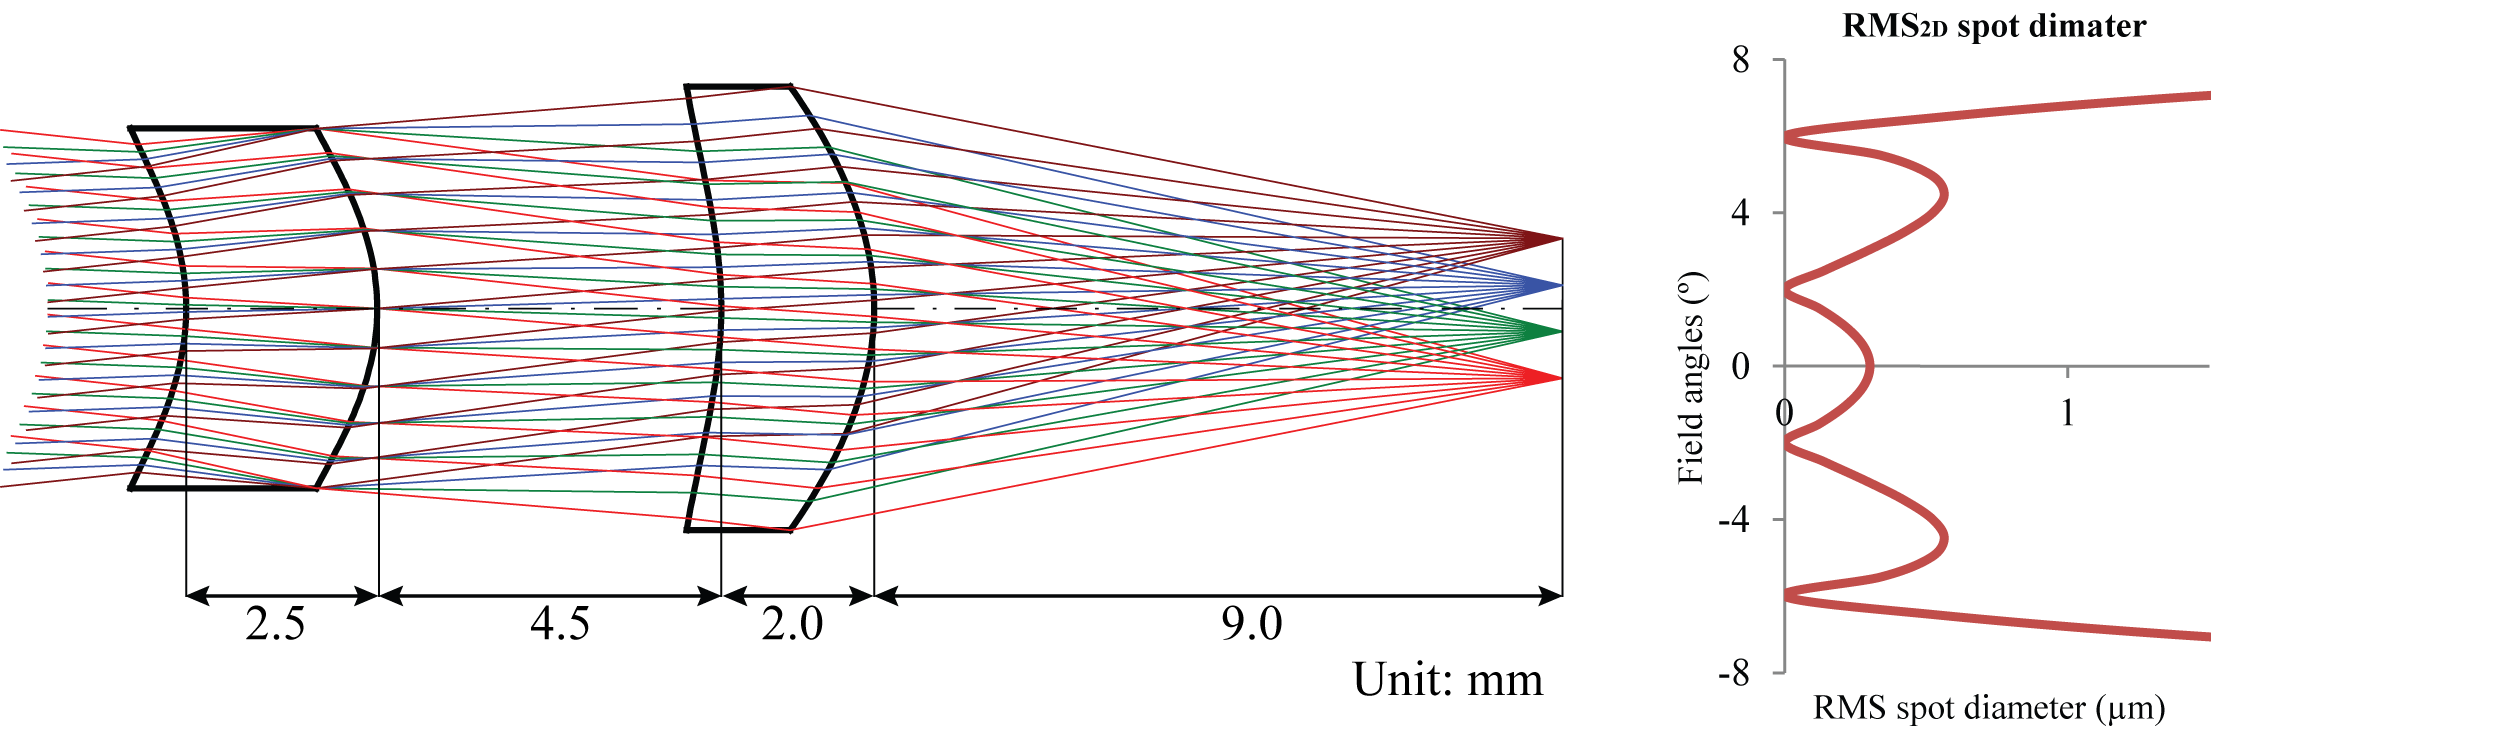
\includegraphics[width=1\textwidth]{chapter-5/figures/Fig2_SMSdesignedSystem.png}
    \caption{SMS 2D design introduced to CODE V after fitting the surfaces to Forbes Qcon polynomials. The change of the spot diameter through the fields is shown on the right side. The four imaging points which are used during the SMS are minimized for their spot diameter. An aperture stop is positioned at the right surface of the first lens element (when counting from left to right).  }
    \label{fig: fig2_SMSdesignedSys}
\end{figure}

\section{Comparing the Results of Different Design Approaches}
Two lens systems were designed and optimized for monochromatic light ($\lambda$= 587.56 nm) using the SMS method and other approaches mentioned in the introduction. Both lenses are made of PMMA (n = 1.4918 at the used wavelength) and have four aspheric surfaces in total. The two systems are referred as system 1 and system 2 where their specifications are given in Table. \ref{table: SMS_SystemSpec}. The object is located at infinity. System 1 has both a smaller field of view (FOV) and aperture, and system 2 has both a larger FOV and aperture. 

\begin{table}[h!]
    \renewcommand*{\arraystretch}{1.2}
    \centering
    \captionsetup{justification=centering}
    \caption{System Specification}
    \label{table: SMS_SystemSpec}
    \vspace{-1em}
    \begin{adjustbox}{max width=\textwidth, center}
    \begin{tabular}{m{2cm} >{\centering\arraybackslash}m{3cm} >{\centering\arraybackslash}m{3cm} >{\centering\arraybackslash}m{3cm} > {\centering\arraybackslash}m{3cm}}
   %\begin{tabular}{c[2cm] c[3cm] c[3cm] c[3cm] c[3cm]}
    \hline
     & \textbf{Image F/Number} & \textbf{Effective Focal Length (EFL)} & \textbf{Maximum Half Field of View (MHFOV)} & \textbf{Position of the Aperture Stop}\\
    \hline
    \textbf{System 1} & 2.24 & 8.60 mm & 7.50$^{\circ}$ & 
   \begin{tabular} {l}
   \\ [-1em]
   At surface 2 
  \end{tabular}\\
    [1em] 
    \textbf{System 2} & 1.77 & 10.60 mm & 11.50$^{\circ}$ & Air-space between the two lenses\\
    \hline
    \end{tabular}
    \end{adjustbox}
\end{table}

Three design approaches are used for the comparison: 1) SMS design with a subsequent one-step optimization; 2) optimization from a spherical system and adding aspheric coefficients, either with multiple coefficients in one-step, two-step (each step with multiple coefficients) or one-by-one (stepwise, only one coefficient per step); 3) global optimization with Global Synthesis (GS) in CODE V. Since we do not intend to compare different global optimization algorithms in this paper, we choose for comparison with SMS only GS that is known to perform very well in comparison with other global optimization and search methods in lens design \cite{KuperGO1992}\cite{ShaferComPhy1994}. For comparison, the systems designed all use Qcon polynomials (Appendix \ref{apdx: chapter-5-system-Qcon-polynomial}) to represent the aspheric surfaces. The variables are the curvatures, conic constants and the coefficients of the Qcon polynomials. To better represent the surface constructed by the SMS method, we use up to the 12th order for system 1, and 16th order for system 2. The vertices are fixed in all cases. For non-GS optimization, we use the default CODE V transverse ray aberration merit function (MF). Two types of constraints are used. One is to constrain the effective focal length (EFL), and the other is to keep the normalization radii \footnote{The normalization radius $r_n$ is a parameter defined in Qcon polynomial which is used to normalize the radial distance $r$. The details are given in Appendix \ref{apdx: chapter-5-system-Qcon-polynomial}.} the surfaces to a value exceeding the size of the surface aperture by $5\%$. The local optimization is done within CODE V based on a damped least square method. Vignetting was readjusted every 20 cycles, since the surface shape may vary significantly during the optimization process. Iterations are stopped when the MF value drops to less than $1^{-5} \mu m^2$ (convergence is then assumed). For GS optimization, the same MF and constraints are applied. However, vignetting can only be adjusted after the GS is finished. 

\begin{figure}[h!]
    \centering
    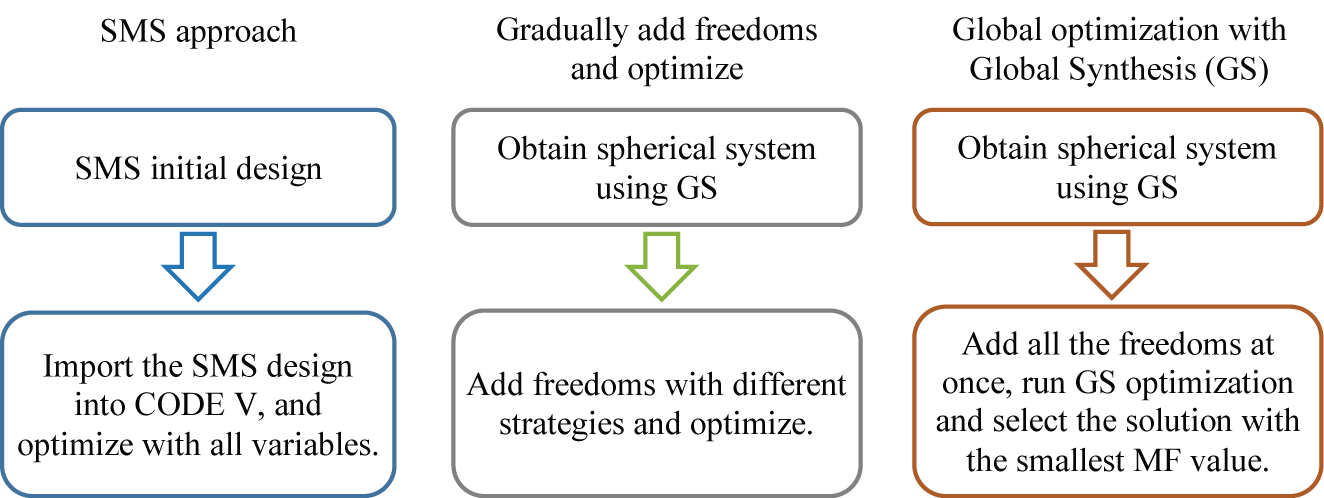
\includegraphics[width=0.8\textwidth]{chapter-5/figures/Fig3_flowchart.png}
    \caption{Flowchart for our different design approaches.}
    \label{fig: fig3_flowchart}
\end{figure}

The SMS 2D procedure enforces stigmatic imaging for meridian rays at a few discrete design fields. After the system is designed with SMS, it is imported into CODE V to be optimized for better performance throughout the whole field of view and the full pupil. The surface parameters of the two SMS constructed systems are given in Table \ref{table: chap5 - sys1 - SMS} and Table \ref{table: chap5 - sys2 - SMS} in the appendix. The left flowchart in Figure \ref{fig: fig3_flowchart} shows the design flow with SMS. 

\begin{figure}[h!]
    \centering
    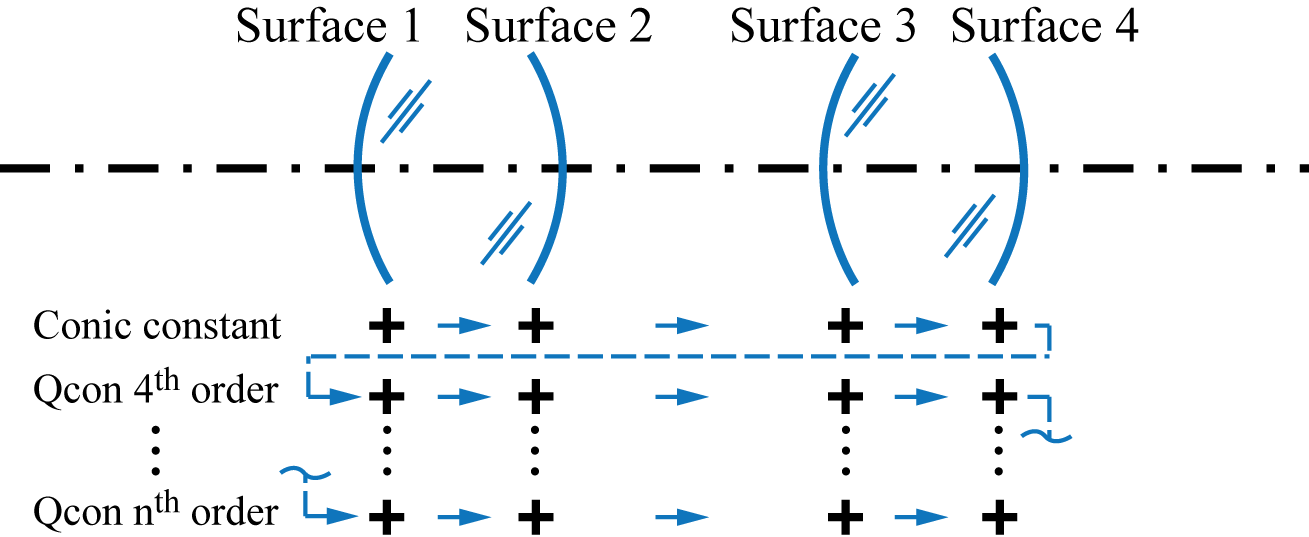
\includegraphics[width=0.8\textwidth]{chapter-5/figures/Figure4_stepwise.png}
    \caption{The strategy for extensive stepwise optimization. The blue shapes represent the optical surfaces. Each cross represents a freedom on the surface described by the Qcon polynomial. The blue arrows indicate how the freedoms are added step by step up to the highest order coefficients used for Qcon polynomials of all surfaces. }
    \label{fig: fig4_stepwiseflow}
\end{figure}


The second approach is conventional and intuitive. We start with a spherical system. The vertices of each surface, the lens thicknesses and air-spaces are fixed. The system specifications shown in Table \ref{table: SMS_SystemSpec} are kept the same for the spherical system. We used the global synthesis (GS) of CODE V to search through the solutions space. It took less than 10 minutes to finish because of the very few number (four) of variables used. Only one solution is obtained. Next, the aspheric coefficients are added as new variables. There are different strategies for adding variables to the system. The direct way is to free all the variables at once and optimize. For an optimization landscape with multiple minima, the optimized solutions will depend on the chosen starting point. Designers will not have control of the optimization route, and it is easy to get trapped in a poor local minimum. A common practice of experienced designers is therefore to add variables step by step. In this chapter, we apply three different strategies for adding new variables: a single-step optimization, a two-step optimization, and an extensive stepwise approach which will be explained below. A two-step approach begins by adding all the conic coefficients at once and then optimize to a local minimum with conic surfaces. Subsequently, the higher-order coefficients of the Qcon polynomials are added all together and optimized. The extensive stepwise approach requires more steps by adding one freedom in each step and then optimize again: We start by freeing the conic constant on surface 1. After optimization, new freedom is added on the next surface. The steps are illustrated in Figure \ref{fig: fig4_stepwiseflow}. A higher-order coefficient is added as variable to surface 1 only after surface 2, 3 and 4 have been given step by step the polynomial coefficient with the same order as variable. The system has been re-optimized in each step. In practice, one can add the new degrees of freedom to the system in different sequences, keeping in mind that on each surface, the coefficients should be added in increasing order. Since it is not known which stepwise strategy will lead to a better solution, in this paper, we choose an easy stepwise strategy for demonstration.  

In addition to the two approaches mentioned above, a global optimization method based on CODE V’s GS is used for comparison as well. The proprietary algorithm of GS can help the designer to automatically explore the solution space and synthesize new configurations from an (almost) arbitrary starting point \cite{codevmanual}. To apply GS, we use the spherical system mentioned above as a starting point. All the degrees of freedom are added at once to the system. GS is executed with constraints on EFL and normalization radii. A time limit of two hours is set to the GS (i. e. GS stops after two hours if it is not finished). The resulting system with a reasonable system shape and the smallest MF value is chosen for the comparison. 

\begin{figure}[h!]
    \centering
    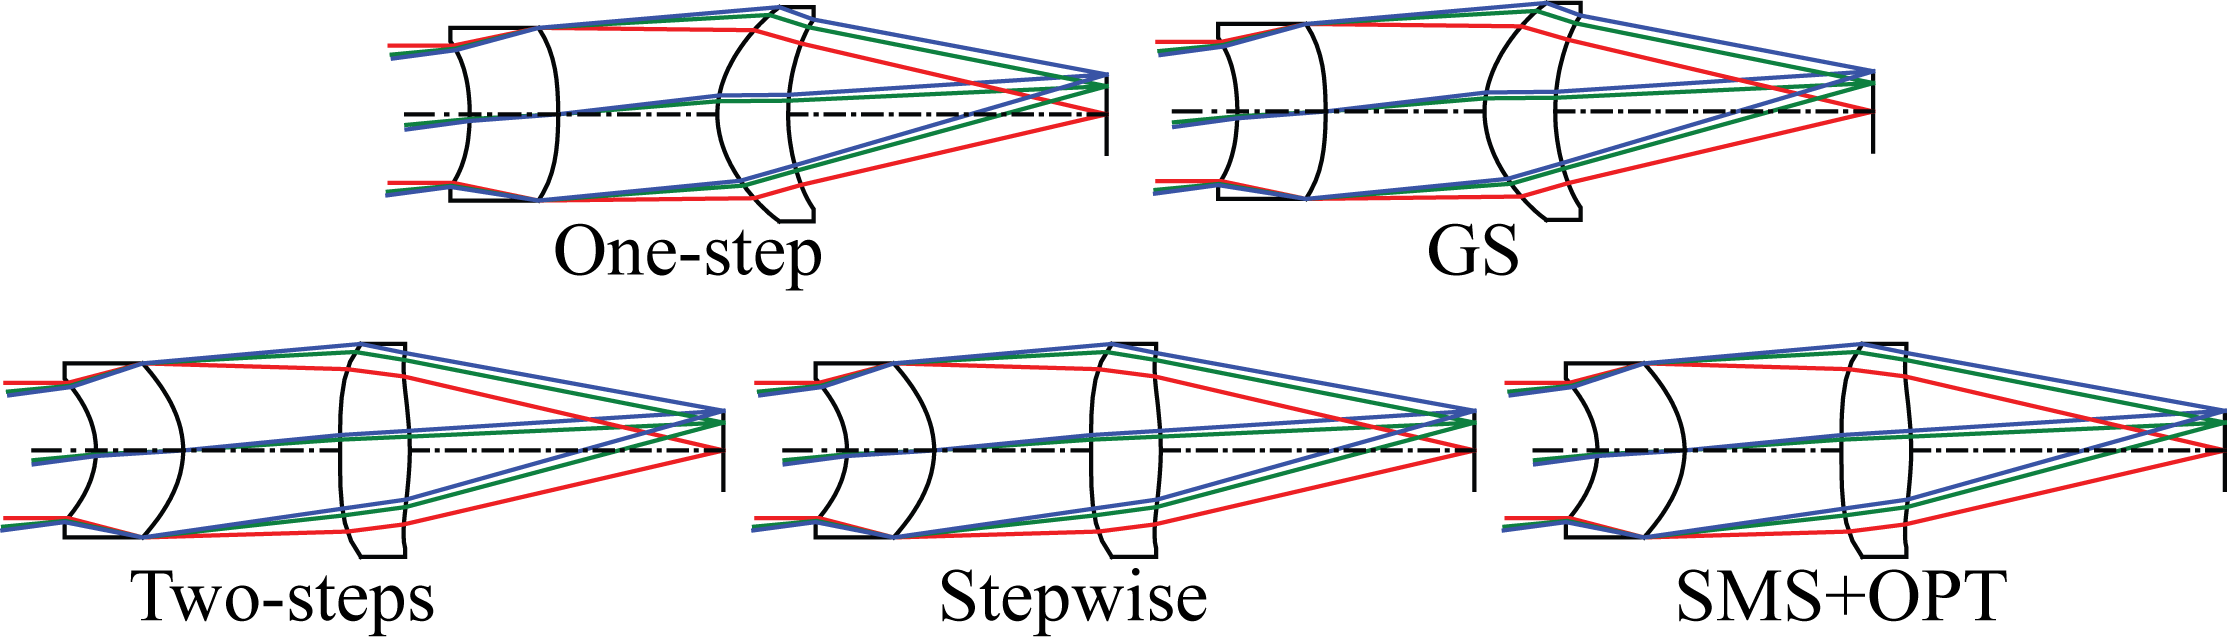
\includegraphics[width=0.8\textwidth]{chapter-5/figures/Figure5_system_plot.png}
    \caption{System 1: the system shapes obtained using different design approaches.}
    \label{fig: fig5_case1_systemplot}
\end{figure}


\begin{figure}[h!]
    \centering
    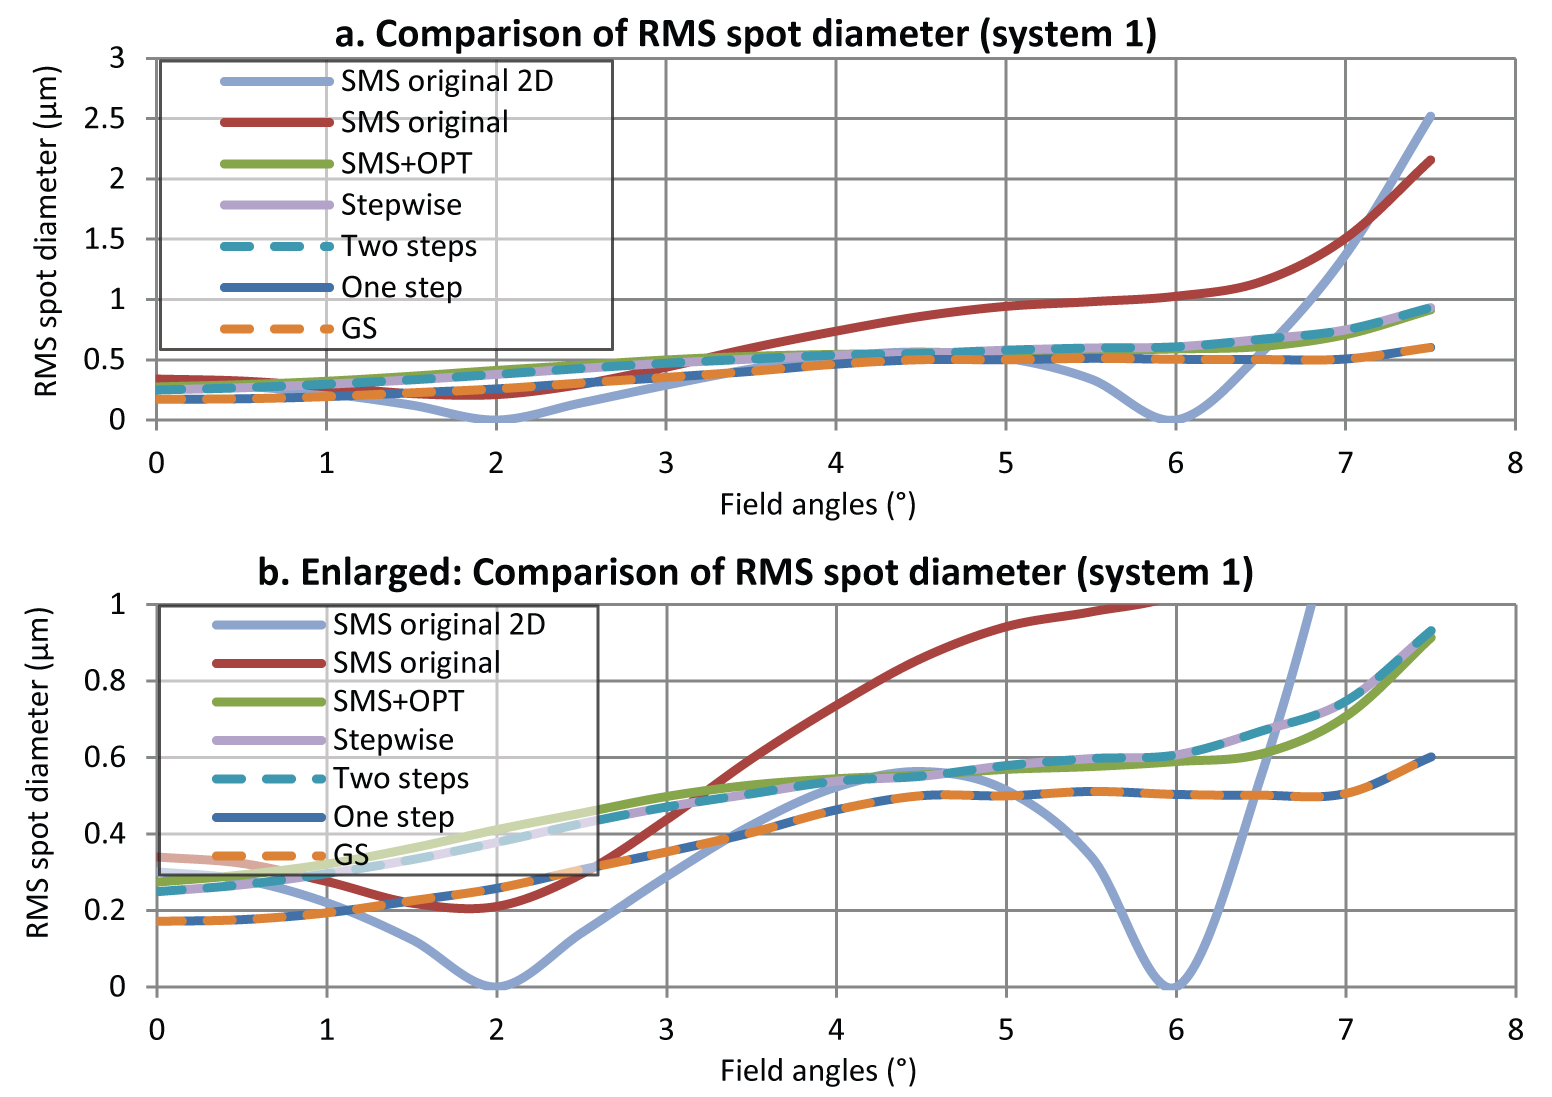
\includegraphics[width=1\textwidth]{chapter-5/figures/Figure6_case1_rmsCurve.png}
    \caption{RMS spot diameter distribution curves for different design approaches: complete curves (a); enlarged vertical axis (b). The RMS spot diameter values of the starting spherical system vary from 60 to 96 µm and are not shown in the graph.}
    \label{fig: fig6_case1_RMScompare}
\end{figure}
\subsection{System 1}
The designed results for system 1 are presented in Figure \ref{fig: fig5_case1_systemplot}. By examining the shapes of the surfaces, we observe two groups of systems: the first group consisting of the solutions obtained by GS and one-step optimization and the second group consisting of the solutions obtained by the two-step, stepwise and the SMS+OPT approaches. This is consistent with the two groups of RMS spot curves in Figure \ref{fig: fig6_case1_RMScompare}. It indicates that the solutions from five different strategies end in two different minima in the design space.

In Figure \ref{fig: fig6_case1_RMScompare}, we see that all five systems generated by the different approaches show good performance with the maximum RMS spot diameter smaller than 1 $\mu m$ at the field of 7.5°. The starting SMS system has a relatively large RMS spot diameter when the field is increased. Since SMS 2D construction involves only meridional rays, the RMS spot diameter is zero for the design fields ( 2° and 6°) only for those meridional rays (SMS original 2D curve in Figure \ref{fig: fig6_case1_RMScompare}). In Figure \ref{fig: fig6_case1_RMScompare}, a minimum is observed at 2° for the SMS original curve, however, at 6° there is no obvious minimum. Since the RMS spot diameter of SMS original in Figure \ref{fig: fig6_case1_RMScompare} results both from meridional and skew rays, it is reasonable to expect that when the whole pupil is considered, skew rays start to have a larger influence on the spot diameter. The optimization of the system constructed by the SMS balances the spot diameter over the field by considering the rays from the whole pupil. Except the SMS original and SMS original 2D curve, the curves in Figure \ref{fig: fig6_case1_RMScompare} form two groups, with GS and one-step forming one group, and SMS+OPT, two-step and stepwise forming the other group, as expected from the system drawings shown in Figure \ref{fig: fig5_case1_systemplot}. The results from GS and one-step group are slightly better than the results of the other group.  It can be observed that the curves of GS and one-step almost overlap. The same happens for two-step and stepwise curves in the second group. The overlap of the curves indicates that the optimization strategies lead to the same local minimum in the optimization landscape. The curve of SMS+OPT only has a very small difference in field dependence of the RMS compared to the stepwise and two steps curves, and therefore can be considered to correspond to the same local minimum. Because of the smaller values of aperture and field considered here, we have many degrees of freedom, and it is easy to achieve diffraction limited performance. In this situation, several good minima exist in the solution space as illustrated in Figure \ref{fig: fig7_landscape_illus}. Even though the designer still has no control during a one-step optimization, the chance for the optimization reaching a good minimum is higher than in a more difficult design problem.

\begin{figure}[h!]
    \centering
    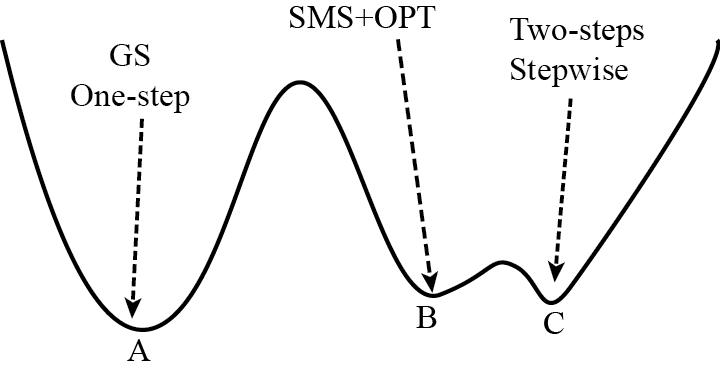
\includegraphics[width=0.6\textwidth]{chapter-5/figures/Fig7_Landscape_illustration_sys1-2.png}
    \caption{An illustration of the design landscape for system 1. We have found three equally good local minima which form two groups. Solution A (MF 0.0301) forms the first group. Solution B (MF 0.0461) and Solution C (MF 0.0450) form the second group.}
    \label{fig: fig7_landscape_illus}
\end{figure}


Figure \ref{fig: fig7_landscape_illus} shows a comparison between the efficiency of the strategies considered in this chapter. The GS result is not included because of its very different approach compared to the others: instead of optimizing from one starting point, it searches for different starting points, applies local optimizations to them, and produces multiple solutions \cite{codevmanual}. We then usually choose the system with the smallest merit function value and perform an extra local optimization to make sure that it converges. In this case, we cannot easily use the number of optimization cycles to represent the efficiency of GS. Three solutions were generated with GS after two hours (Intel i5-3470 dual-core @3.20 GHz system). In comparison, it took around 30 seconds for a one-step optimization to run 1000 cycles on the same computer. In Figure \ref{fig: fig8_case1_efficiencyCompare}, the starting points are shown at cycle 0. The two groups have their average MF values as 0.0454 and 0.0301(the MF value of the GS result is 0.0301). An MTF analysis shows that all five systems are diffraction limited at the wavelength used here. This is consistent with our statement that the design problem is easy and multiple equally good minima are present. Therefore, this example shows that in simple design problems like system 1 simple methods can easily lead to a good solution. 

\subsection{System 2}
System 1 has a relatively small pupil and field, which reduces the difficulty of the design. With the same approach, we used SMS to construct system 2, which has both a larger pupil and field of view. Figure \ref{fig: fig9_case2_systems} shows the five plots of the systems produced by the five mentioned optimization approaches. In contrast with the solutions of system 1 in Figure \ref{fig: fig5_case1_systemplot}, four different system shapes are now obtained, where stepwise and SMS+OPT resulted in the same system shape. The operation with GS for system 2 was not as straightforward as that for system 1 which will be explained below. It is also worth noting that the aperture stop of system 2 is placed in between the two lens element as shown in Figure \ref{fig: fig9_case2_systems}. This is to impose the requirement that, when using SMS, only four ray bundles are used for a four-surface design. It turned out that other positions of the aperture stop will lead to the use of more than four ray bundles which will not be consistent with the SMS design approach in system 1. In system 1, four ray bundles (on the left-hand of  Figure \ref{fig: fig2_SMSdesignedSys}) are used to construct four surfaces. The result is that four points have zero RMS spot diameter at the image plane (on the right-hand of Figure \ref{fig: fig2_SMSdesignedSys}). It is demonstrated in the previous research \cite{BenitezSPIE2014}\cite{FDuerrOE2013}\cite{FDuerrOE12} that given certain conditions, it is possible to use more than N ray bundles to construct N optical surfaces using the SMS method. This is realized by adjusting the size of the aperture stop or the distance between the aperture stop and optical surfaces. As a result, the footprints of the original design ray bundles can leave unoccupied patches on optical surfaces. These unoccupied patches can be used to couple additional ray bundles.   

\begin{figure}[h!]
    \centering
    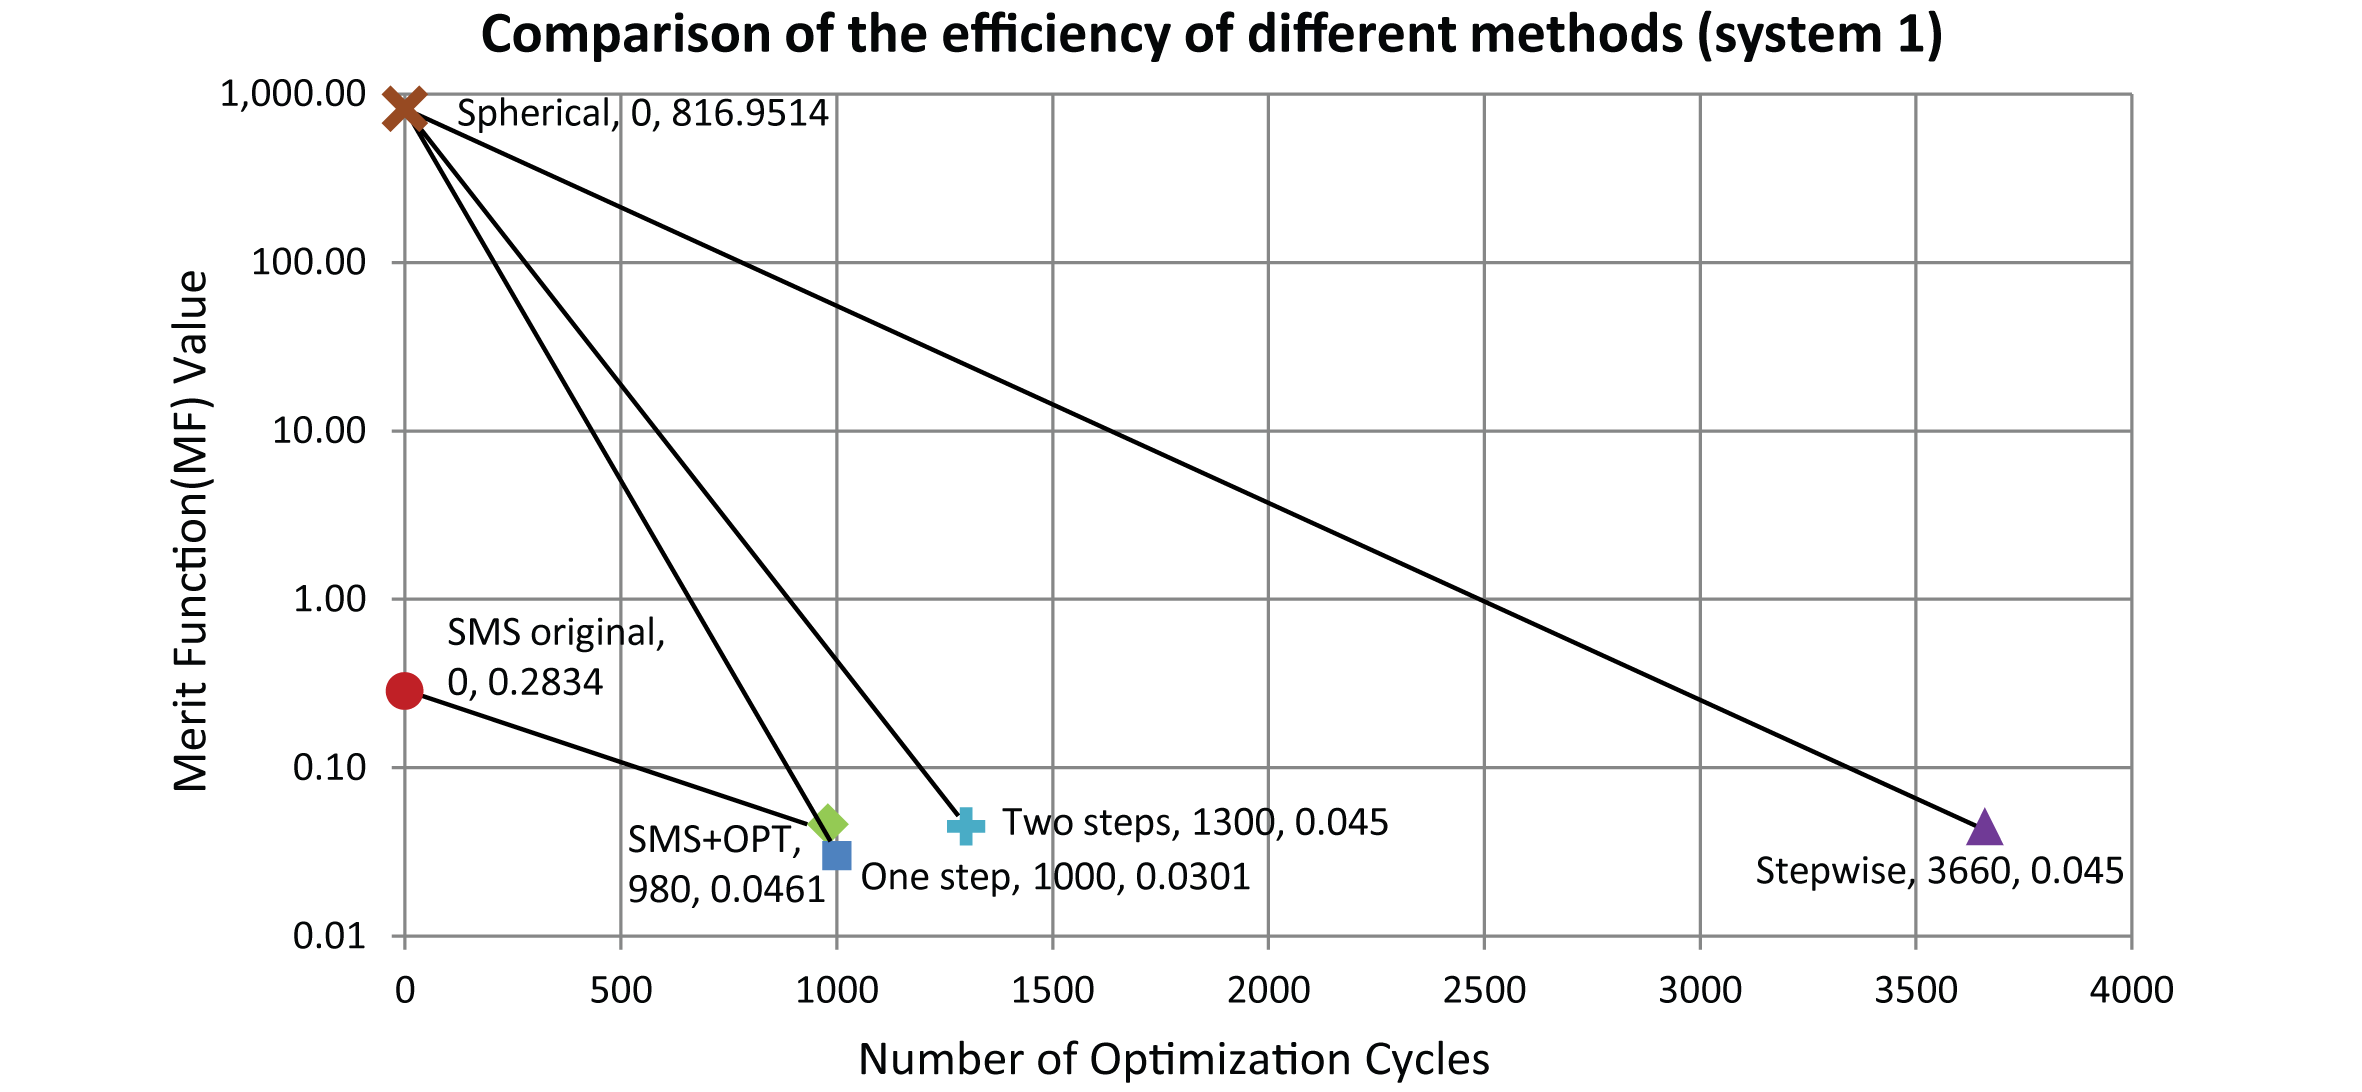
\includegraphics[width=1\textwidth]{chapter-5/figures/Figure8_OE340147.png}
    \caption{Comparison of the efficiency of different design methods analyzed, evaluated as the merit function value versus the number of cycles performed. The merit function value of the system obtained with GS is 0.0301.}
    \label{fig: fig8_case1_efficiencyCompare}
\end{figure}

Optimization with conic constants as variables ended with systems having an extremely large conic constant. Therefore, we first fixed the conic constant on all the surfaces to $-1$, and ran the GS which resulted in twelve solutions. After that, the conic constants on all the surfaces of the twelve systems were freed at once as variables. Subsequent local optimization, which is the same as the one used in the other four strategies, was applied to each of the twelve systems. The system with the smallest MF value was chosen as the final result. In Figure \ref{fig: fig10_case2_rmsCurvecompare}, the curves of the RMS spot diameter as function of the field angle can be again divided into two groups. One-step and two-step optimization generate poorer solutions than the other three approaches. SMS with optimization, stepwise optimization and GS obtain good solutions with close RMS dependence over the field (Figure \ref{fig: fig10_case2_rmsCurvecompare}(b)). Consistent with the same system shape in Figure \ref{fig: fig9_case2_systems}, the RMS curves of SMS+OPT and stepwise in Figure \ref{fig: fig10_case2_rmsCurvecompare} almost overlap with each other. On the other hand, the result of GS with a different system shape produces a different RMS curve, where the RMS spot diameter is bigger under 7.8° and smaller above 7.8°.

\begin{figure}[h!]
    \centering
    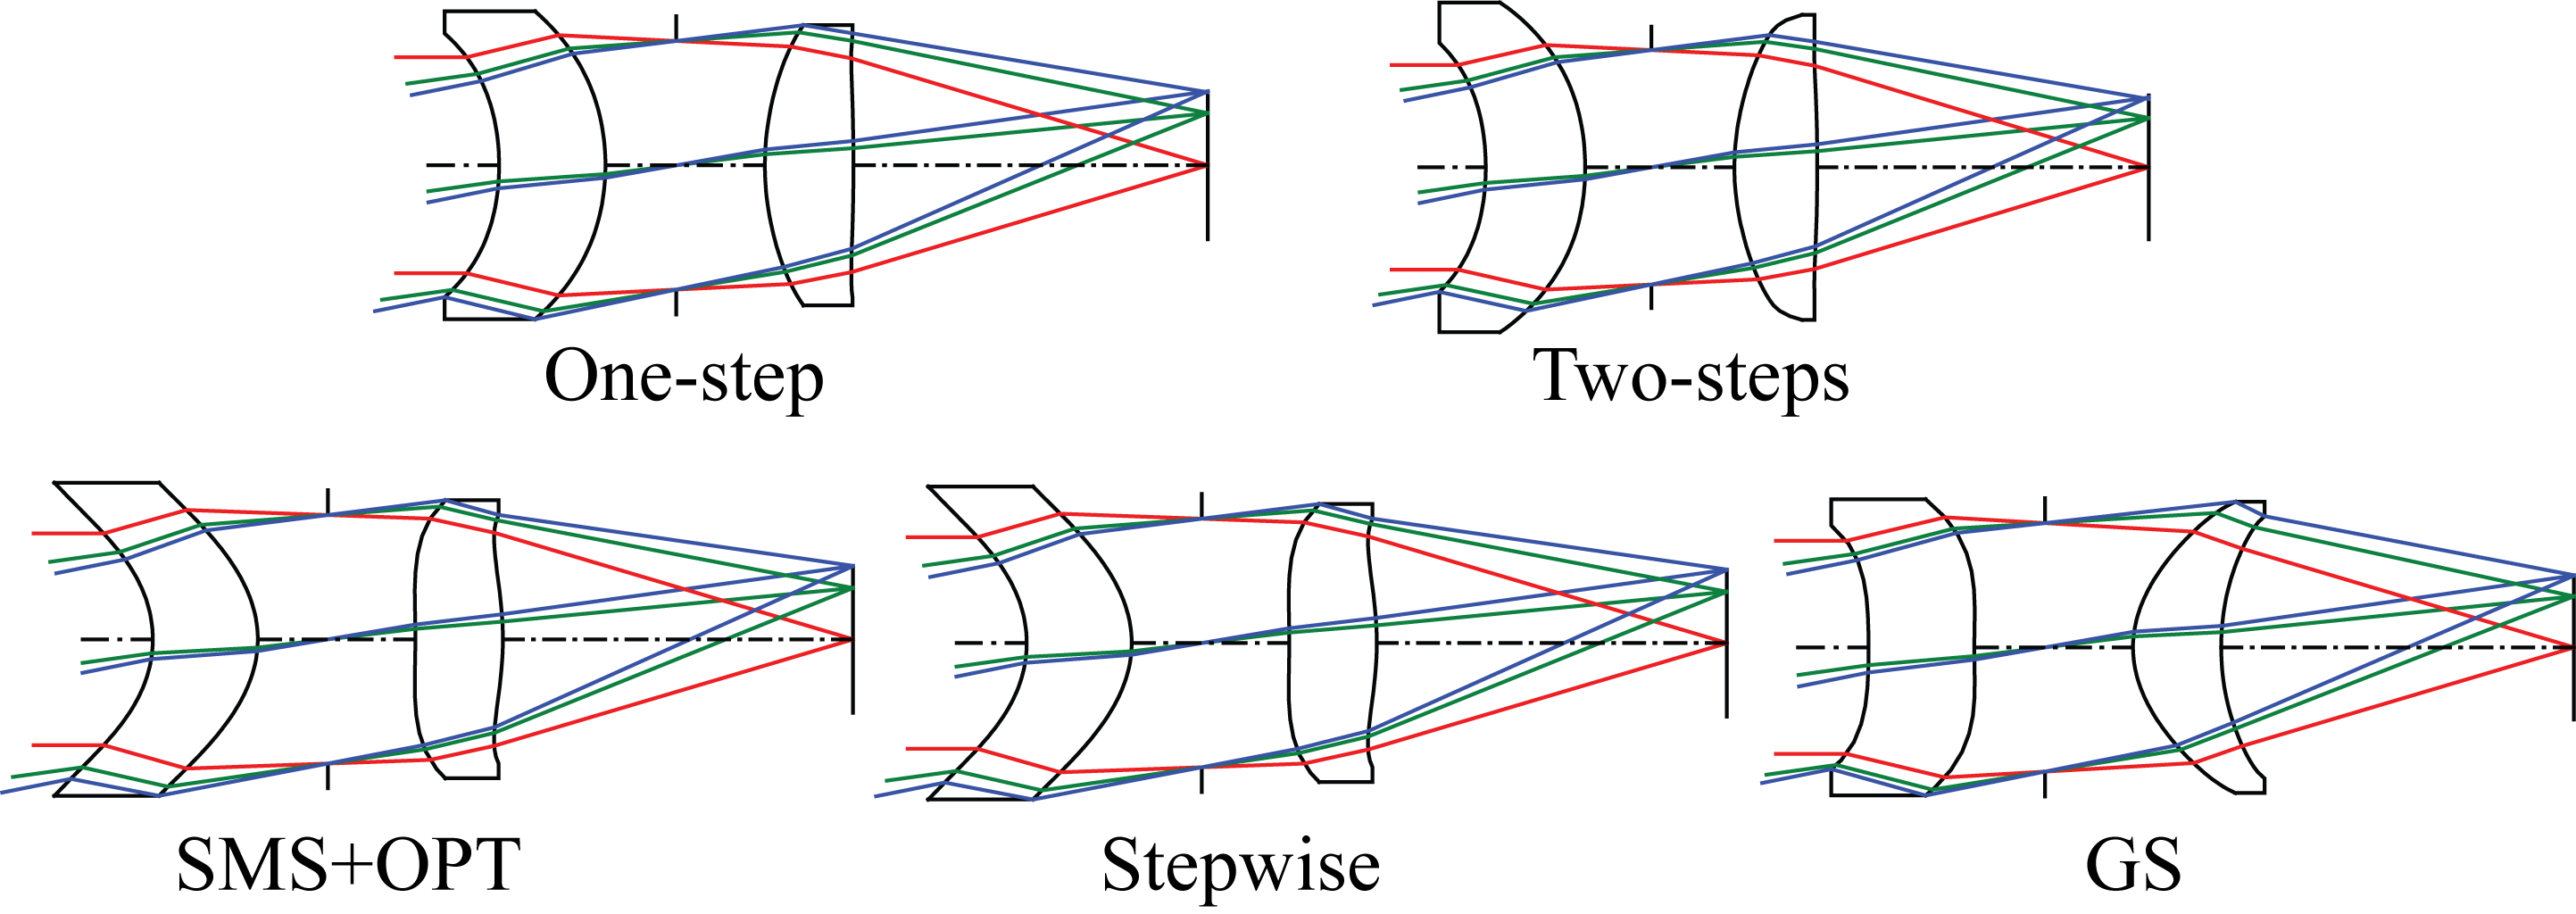
\includegraphics[width=0.8\textwidth]{chapter-5/figures/Figure9_system2_solutions.png}
    \caption{System 2: the system shapes obtained using different design approaches.}
    \label{fig: fig9_case2_systems}
\end{figure}

Figure \ref{fig: fig11_case2_efficiencyCompare} shows the comparison of the efficiency of different methods. Stepwise needs a large number of optimization cycles (8100 cycles) to converge. With a similar merit function value, fewer optimization cycles are needed for SMS optimization. This shows the SMS constructed starting point is closer to the minimum in the optimization landscape. Both one-step and two-step optimization are trapped in poor solutions with MF values at least nine times of the best solution. 
From the two examples we studied, to design a simple system with small field and aperture, all approaches including a one-step optimization were able to obtain good solutions. However, when the field and aperture increased, simple strategies like one-step and two-step started to fail by getting trapped in poor local minima as shown in the example of system 2. A stepwise approach leads to a good local minimum with a large number of optimization cycles. An SMS constructed starting point located closer to a good solution shows its advantage in both cases where fewer optimization cycles are needed to reach a good local minimum.

\begin{figure}[h!]
    \centering
    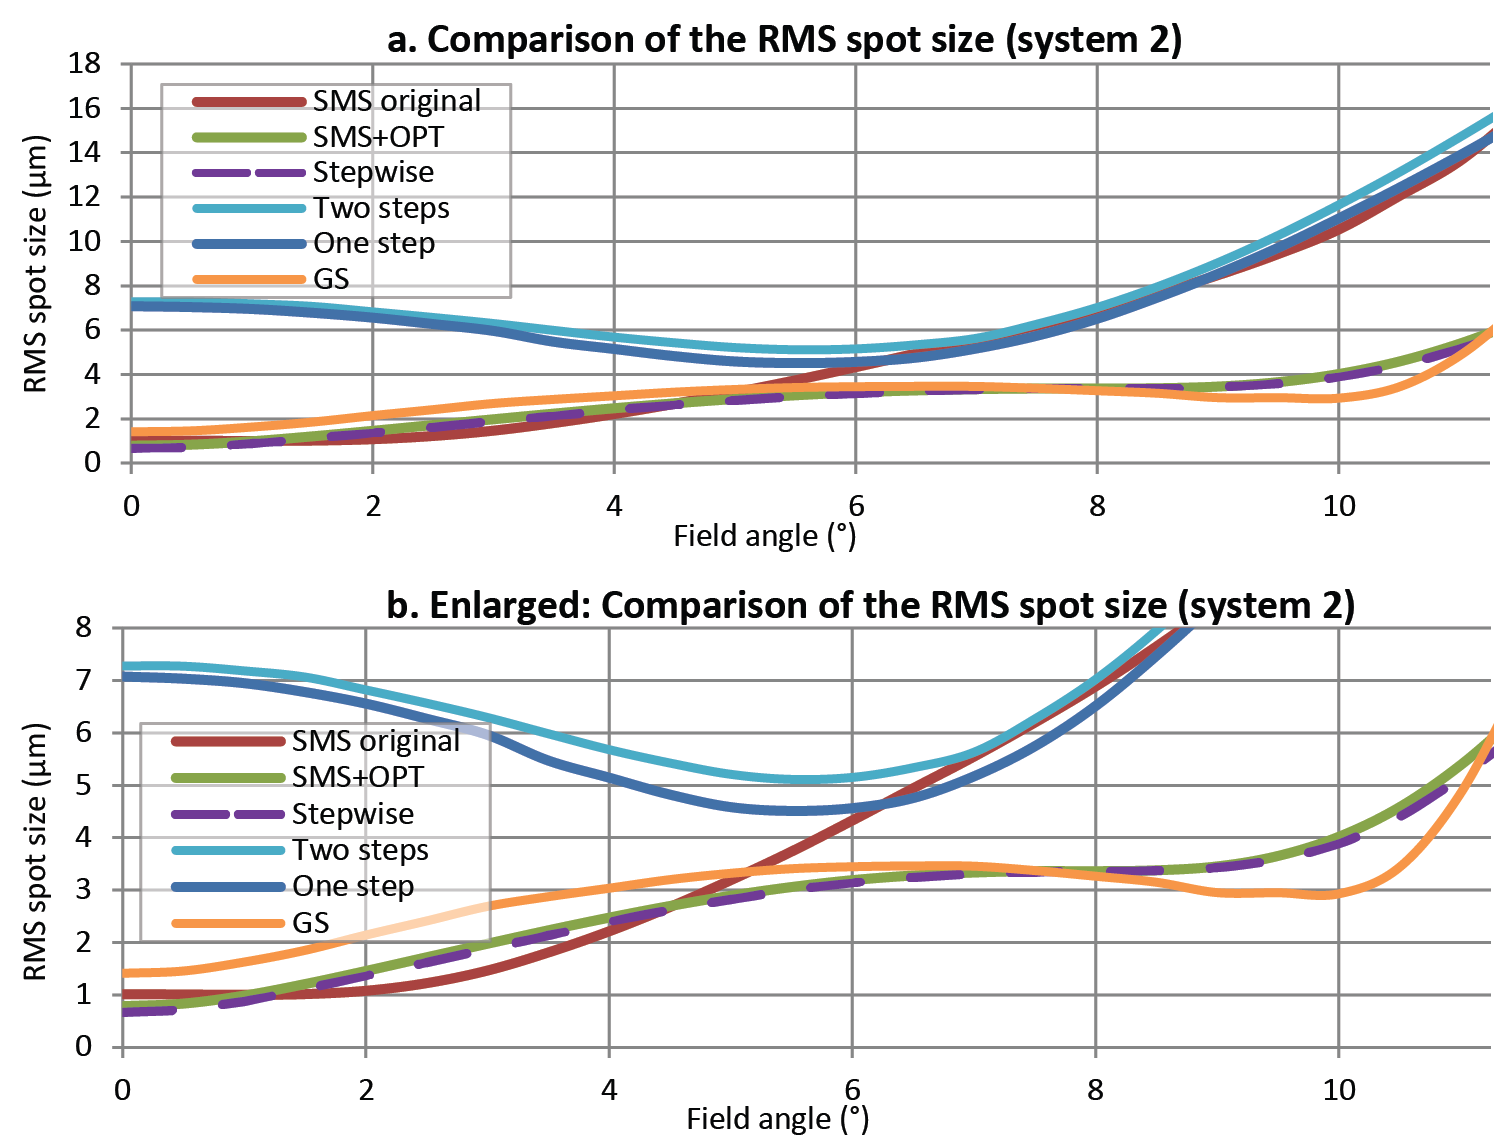
\includegraphics[width=1\textwidth]{chapter-5/figures/Fig10_case2_rms.png}
    \caption{RMS spot diameter curves for system 2 using different design approaches: complete curves (a); enlarged vertical axis (b). The RMS spot diameter values of the starting spherical system vary from 124 to 142 µm from the center to the full field and are not shown in the graph.}
    \label{fig: fig10_case2_rmsCurvecompare}
\end{figure}

\begin{figure}[h!]
    \centering
    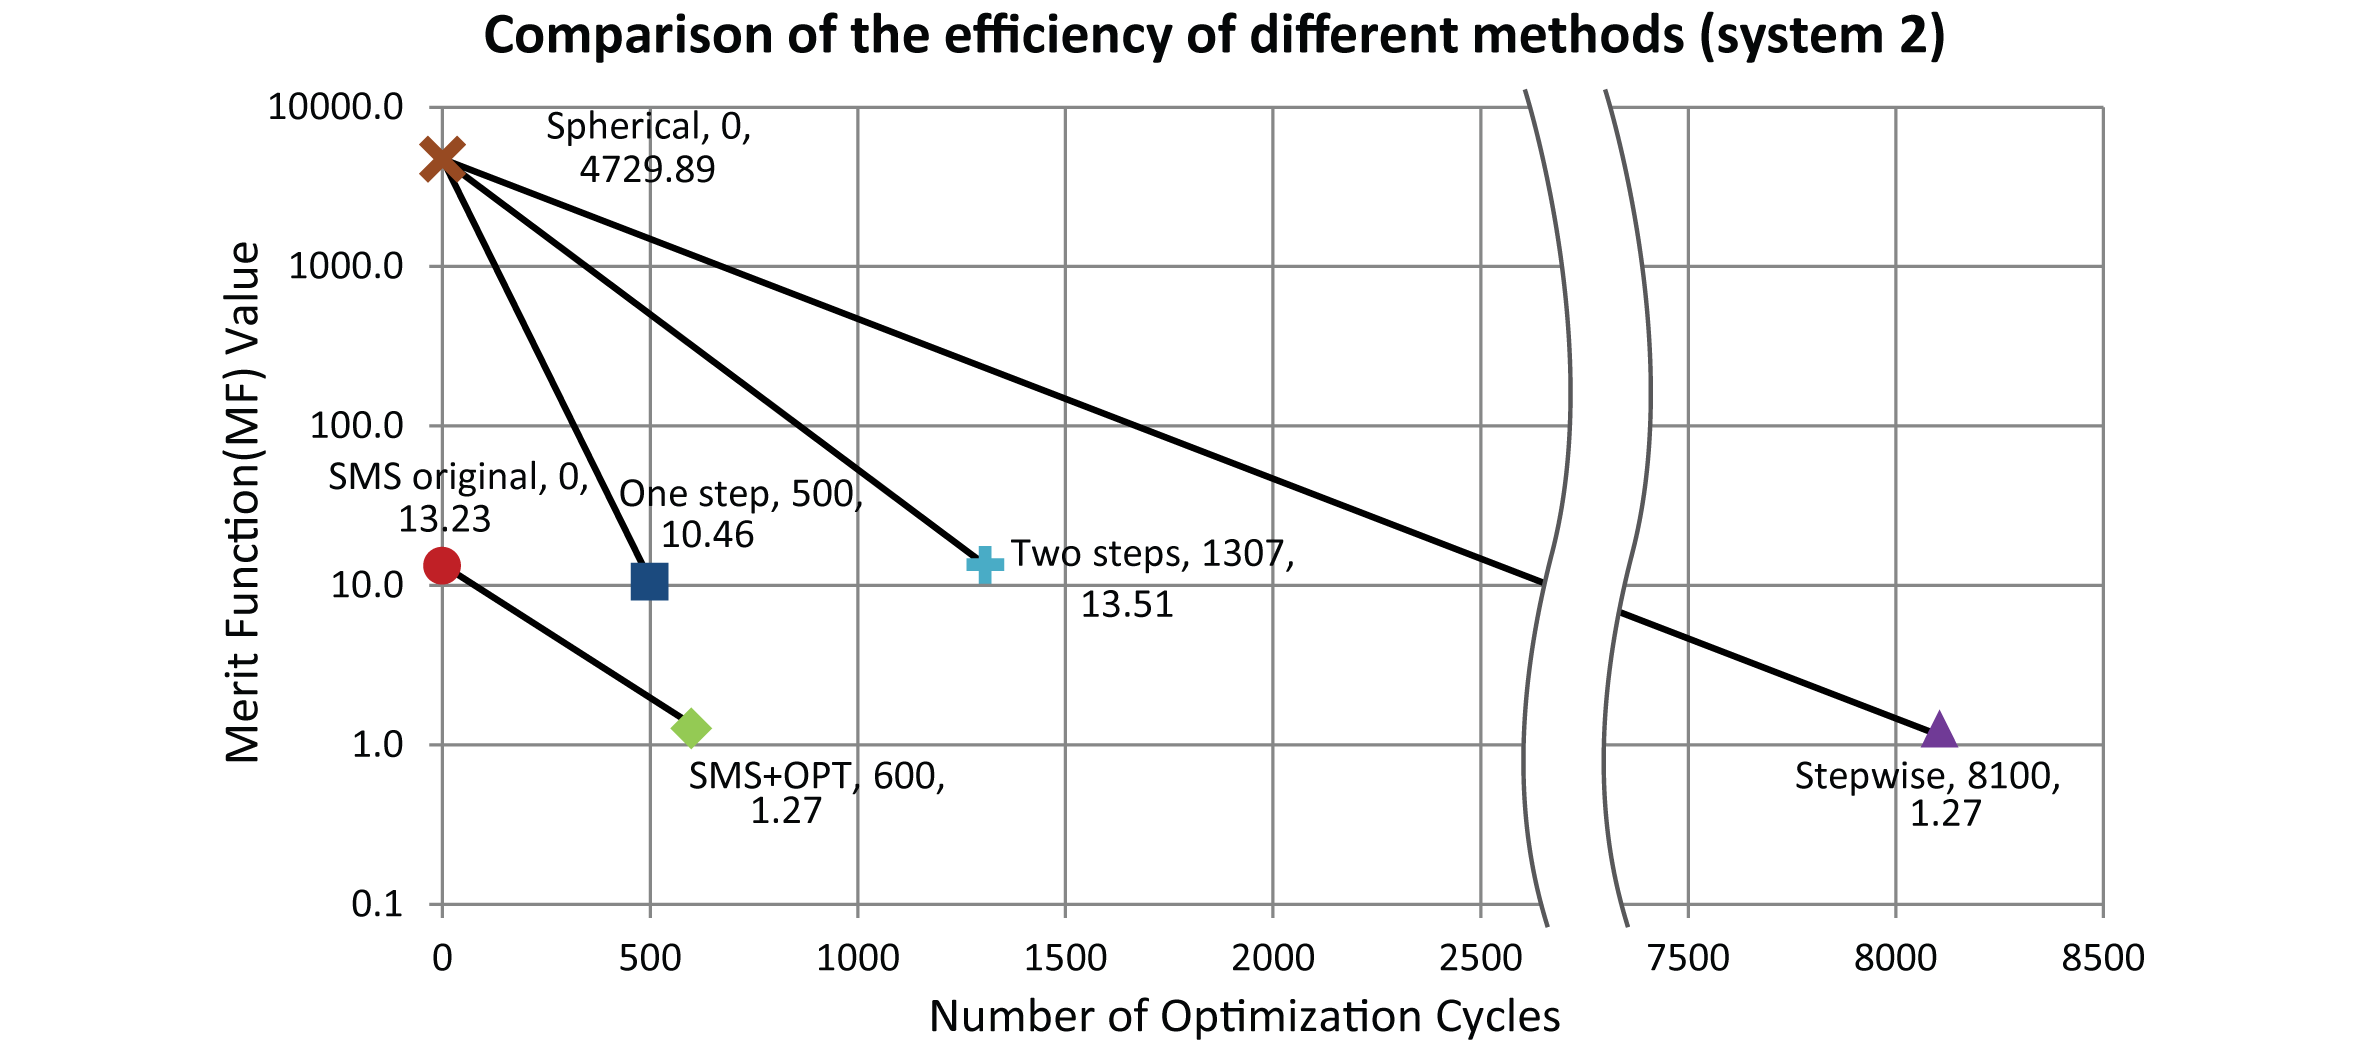
\includegraphics[width=1\textwidth]{chapter-5/figures/Figure11_OE340147.png}
    \caption{Comparison of the efficiency of different design methods. The starting points are shown at zero cycles and are connected with the straight lines with the results obtained using different design methods. The merit function value of the GS result is 1.03.}
    \label{fig: fig11_case2_efficiencyCompare}
\end{figure}
\newpage
\section{Design Landscape for Aspheric Systems}
In our examples, we have noticed that when aspheric variables are not introduced, there is only one solution in the optimization landscape given the boundary condition for rays that are traced. However, when aspheric coefficients are added, new minima start to appear. 

\begin{figure}[h!]
    \centering
    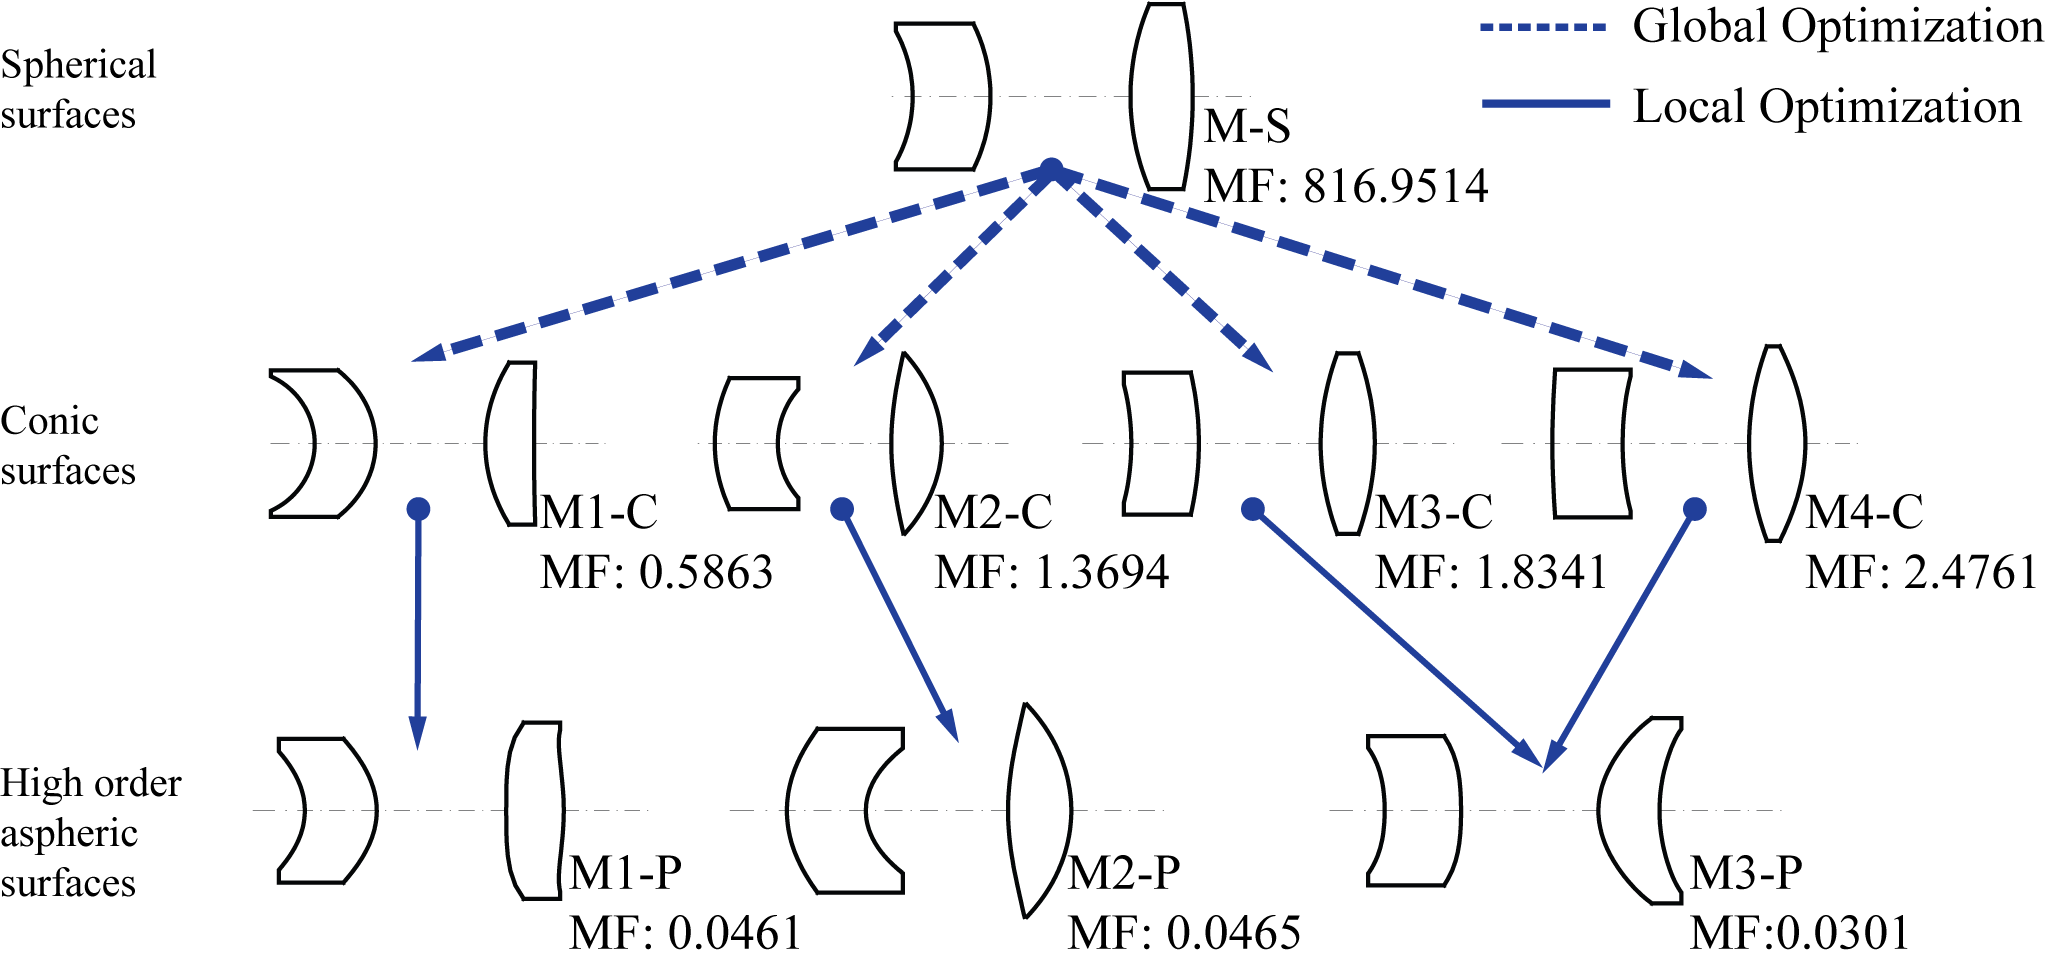
\includegraphics[width=0.8\textwidth]{chapter-5/figures/Fig12_System1_structure.png}
    \caption{Evolution of the minima with the change of aspheric coefficients for system 1. Four minima are found with conic surfaces. They become three minima when optimized with aspheric coefficients up to 12th order. All three solutions have been obtained with the approaches we mentioned previously. M1-P and M3-P are the two solutions identical to the ones shown in Figure \ref{fig: fig5_case1_systemplot}. M2-P is one the results obtained by GS (not the best in terms of merit function value). }
    \label{fig: fig12_case1_optStruc}
\end{figure}

After adding the conic constant as a variable, multiple minima appear in the design landscape. We used the GS of CODE V in this case to search for different solutions. For system 1, we have found four minima (Figure \ref{fig: fig12_case1_optStruc}), and for system 2 three (Figure \ref{fig: fig13_case2_optStruc}). 
The following step consisted of adding all other higher-order aspheric coefficients at once and locally optimizing the systems from the conic minima. For system 1, four different minima in conic space converge to three minima. In Figure \ref{fig: fig12_case1_optStruc}, two of the three minima (M1-P, M3-P) are identical to the ones shown in Figure \ref{fig: fig5_case1_systemplot}. M2-P was one of the results obtained with the GS that is not shown in Figure \ref{fig: fig5_case1_systemplot}. GS generates multiple solutions at once and the one with the smallest merit function is chosen. For system 2, three solutions result from the three conic minima. In Figure \ref{fig: fig13_case2_optStruc}, M1-P and M2-P are same as the results of the two-step approach and the SMS with optimization, respectively. M3-P is a local minimum which is not found by the previously discussed five approaches we used. In terms of merit function value, M3-P is almost seven times of M2-P (the smallest merit function found), and approximately two-third of M1-P.

\begin{figure}[h!]
    \centering
    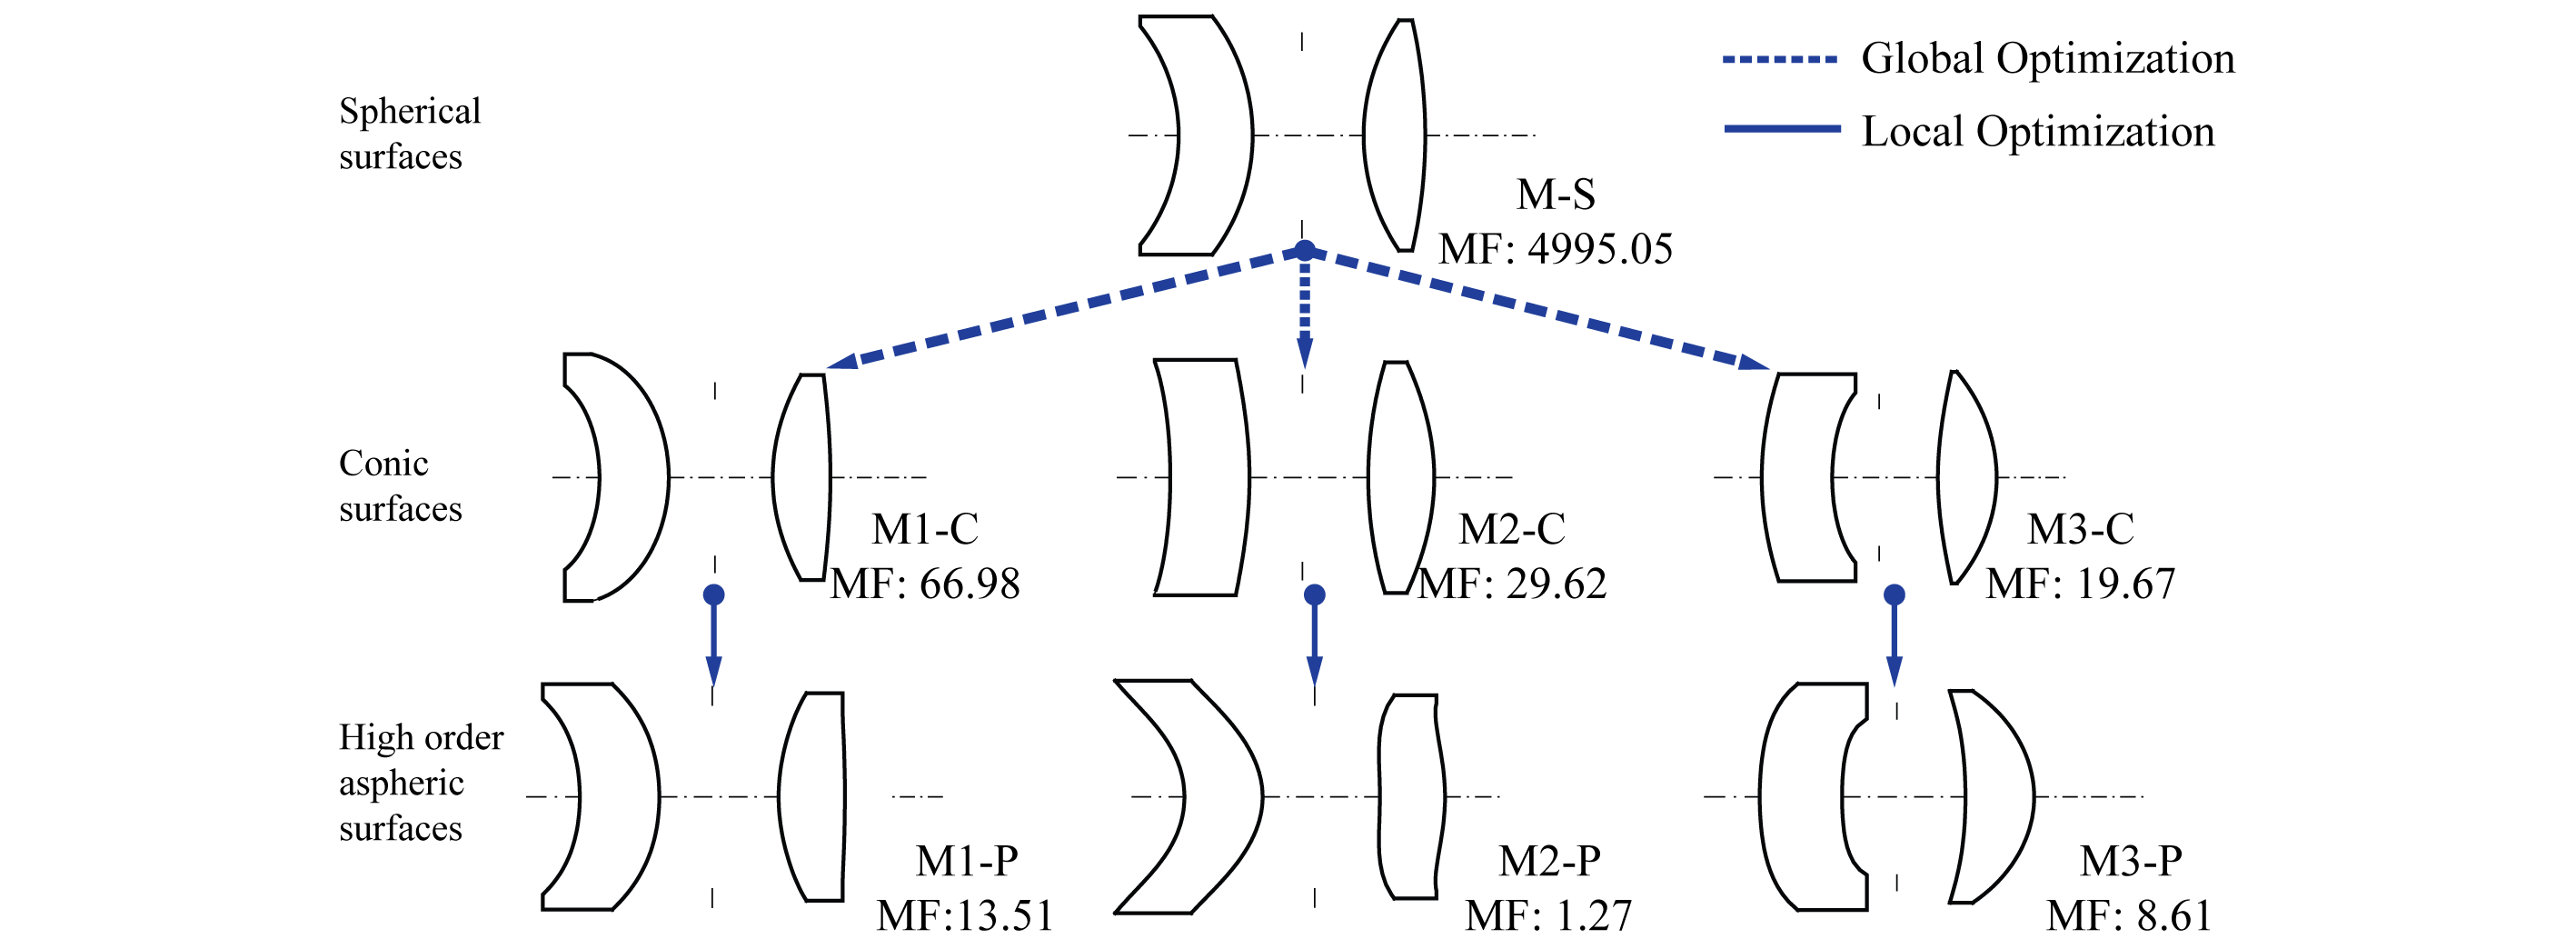
\includegraphics[width=1\textwidth]{chapter-5/figures/Fig13_OE340147.png}
    \caption{Figure \ref{fig: fig13_case2_optStruc}. Evolution of the minima with the change of aspheric coefficients for system 2. Three minima are found with conic surfaces. Adding higher-order aspheric coefficients up to 16th order to these minima results in three different solutions. M1-P is the solutions that is also found by the two-step approach, and M2-P is the solution that is also found by the SMS with optimization in Figure \ref{fig: fig9_case2_systems}}
    \label{fig: fig13_case2_optStruc}
\end{figure}

The results show the dynamic behavior of the optimization landscape, namely, the number of minima depends on the number and type of variables used. In the two systems we have studied in this chapter, the introduction of the conic surface creates new minima in the design landscape, and adding higher-order aspheric coefficients deepens the original minima. For a simple system, adding higher-order aspheric coefficients does not complicate the landscape. With local optimization, the conic solutions lead to the good solutions with higher-order aspheric coefficients. In the case of system 2 where aperture and field are large, however, adding higher-order aspheric coefficients complicates the landscape by creating new local minima. That is the reason why simple strategies are trapped in poor local minima. In both cases, the SMS constructed starting points are already close to one of the good local minima in the landscape. Therefore, local optimizations with few optimization cycles lead to good solutions if as starting value the system constructed with SMS is used.

\section{Conclusions}

Two different optical systems comprising of two lenses were analyzed. In the analysis of the design landscape of the systems, we have observed that with aspherising the surfaces, new minima emerge into the landscape. In both examples, introducing lower order aspheric coefficients (conic constant) to all the surfaces brings new local minima into the landscape, and adding higher-order aspheric coefficients deepens the minima. In a simple design with both small aperture and field (system 1), adding higher-order coefficients does not complicate the landscape by creating new local minima. In contrast, for a different design with large aperture and field (system 2), higher-order aspheric coefficients introduce new local minima, where a design process can be trapped.

We have compared the SMS design approach with other design techniques for both system 1 and system 2. In the case of system system 1 which is relatively simpler, all design techniques including a one-step optimization found solutions close to the diffraction limit. Nevertheless, surface shapes of the final designs were different which suggested that their optimization paths ended in different basins of attractions. 

For the case of system 2, SMS with posterior optimization, the stepwise approach and GS found optimal solutions, while one-step and two-step approach only obtained pool local minima. After carefully analyzing the three obtained results, we conclude that they belong to two different minima. Since designing system 2 is more demanding than system 1, less robust methods such as one-step optimization and two-step optimization did not lead to good minima. Despite that three approaches found good solutions, stepwise optimization usually takes the largest amount of optimization cycles. GS works well for the simple case. However, for system 2, effective constraints (in this case, fixed conic constant) and further optimizations had to be implemented into GS to get reasonable solutions. 

In practice, lens design problems are very different depending on the application and constraints. While we cannot guarantee that SMS will find good solutions in other design problems, the present results are encouraging. In both design problems system 1 and system 2, SMS with posterior optimization gives good solutions and we can see from Figure \ref{fig: fig8_case1_efficiencyCompare} and Figure \ref{fig: fig11_case2_efficiencyCompare} that in the two examples considered, SMS constructs good starting points which are already close to the good solutions. We believe that with this and similar comparative studies, new insight can be obtained about the characteristics of different design methods. 


\references{dissertation}

